\documentclass[conference]{IEEEtran}
\IEEEoverridecommandlockouts
% The preceding line is only needed to identify funding in the first footnote. If that is unneeded, please comment it out.
\usepackage{cite}
\usepackage{amsmath,amssymb,amsfonts}
\usepackage{algorithmic}
\usepackage{graphicx}
\usepackage{textcomp}
\usepackage{xcolor}
\def\BibTeX{{\rm B\kern-.05em{\sc i\kern-.025em b}\kern-.08em
    T\kern-.1667em\lower.7ex\hbox{E}\kern-.125emX}}
\begin{document}

\title{Property-Based Explainable Artificial Intelligence for Handwritten Digit Classification}

\author{\IEEEauthorblockN{Paul Whitten}
\IEEEauthorblockA{\textit{Electrical, Computer, and Systems Engineering(ECSE)} \\
\textit{Case School of Engineering (CSE)} \\
\textit{Case Western Reserve University(CWRU)} \\
Cleveland, OH, USA \\
0000-0002-7787-473X}
\and
\IEEEauthorblockN{Francis Wolff}
\IEEEauthorblockA{\textit{ECSE} \\
\textit{CSE} \\
\textit{CWRU} \\
Cleveland, OH, USA \\
fxw12@case.edu}
\and
\IEEEauthorblockN{Chris Papachristou}
\IEEEauthorblockA{\textit{ECSE} \\
\textit{CSE} \\
\textit{CWRU} \\
Cleveland, OH, USA \\
cap2@case.edu}

}

\maketitle

\begin{abstract}
There has been explosive growth of practical AI in recent years.
However, results of AI systems are not readily explainable to humans.
A major concern of current AI systems is an inability to explain decisions.
Explainable artificial intelligence has been posed to mitigate these concerns.
This work is an attempt to explore a methodology that provides explanations
for classification decisions.
\end{abstract}

\begin{IEEEkeywords}
explainable, artificial intelligence, machine learning
\end{IEEEkeywords}

\section{Introduction}

Recent advances in Machine Learning (ML) have brought about wide adoption of ML algorithms for many applications.  Despite various successes, there is a reluctance to adopt ML in some applications because ML behaves like a black box, decision making by the black box is often not explainable to humans.  This working paper approaches the widely studied problem of classifying images of handwritten digits into the ten decimal digit classes, zero through nine, from an Explainable Artificial Intelligence (XAI) perspective.

While we approach XAI for a specific classification problem in the MNIST handwritten digit database, which consists of 28x28 images of handwritten digits into the ten decimal digits, we feel the methodology translates to other problems of explainable classification among a finite set of classes.

We present an iterative methodology using properties of the input data to the classification problem.  This supervised leaning methodology involves the discovery of domain-specific properties of the input data.  Transformation of the input data according to the properties.  Construction and training of distinct property-specific explainable Neural Networks (NNs).  Build an explainable confidence knowledgebase of results from training the property NNs.  The Explainability of eventual results comes from the property-specific NNs and the knowledgebase.  Classification can proceed according to the property NN output.  We pose a weighted voting mechanism based on the knowledgebase as well as an ML approach.   Properties are finally adjusted based on result scoring.

When applying this methodology to the classification problem in the MNIST handwritten digit database, there is a potential for acceptable classification while also providing a means of justification for classification decisions based on the explainable properties.

In addition to providing an explainable justification for classification decisions, multiple simple neural networks in a wide arrangement, like we use in this work, may offer advantages in the simplicity (depth) of the NN architecture and gains in speed over more complex NN architectures.

\section{Related Work}

The ability to map the learning classifier or recognizer to human-based explainability is a challenging task for human understandability.  Currently, there are at least seventeen explainable techniques such as
decision tree-based, rule-based (i.e. knowledge-base), salience mapping,
sensitivity-based analysis, feature importance, fuzzy-based, neural-network, and generic-programming based.  These techniques use one of three basic evaluation approaches: application-grounded, human-grounded and functionally grounded. \cite{Hagras18} \cite{BlackBox18} \cite{Survey18} \cite{Fuzzy19} \cite{GP18}.

\section{Methodology}

 \begin{figure}[htbp]
\centerline{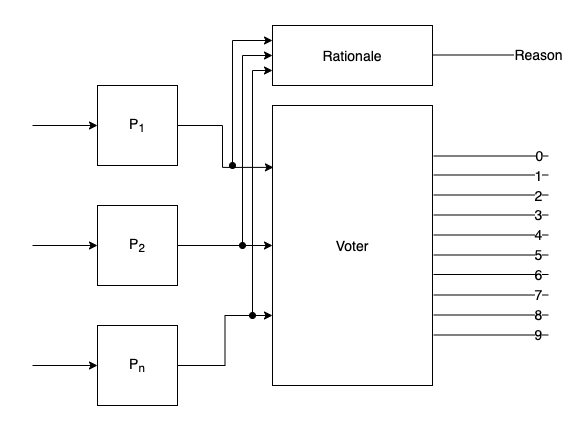
\includegraphics[width=90mm]{./images/voting_prop_nn.png}}
\caption{XAI Methodology Summary}
\label{voting}
\end{figure}

This work aims to pose a means of explaining the classification to a human.  We do not wish to compete with established algorithms that perform exceptionally well in classification of input.   The effort required in applying the methodology in this work is significant compared to training a classifier that will act as a black box, and therefore not be explainable.

Our methodology for explainability is summarized as the use of explainable properties of the input to make distinct classification decisions for each property.  Those distinct classifications are input to a voter to provide the best classification result.  Rationale, based on the explainable properties, are combined with the voter result to provide an explanation. 

The methodology is depicted in Fig.~\ref{voting} where the $P_x$ squares represent logic to make classifications based on properties 1 through n.  The voter is then used to consider each of the choices from the properties and provide the best decision.  The decision is combined with the rationale from the property results to provide an explanation.

Further detailing the decision making process for explainable properties, we considered how explainable properties could be mapped to the input.  In this work we give examples of input transformations related to explainable properties that aid in classification while providing human understandable rationale for classification decisions.  This is depicted in Fig.~\ref{proptrans} where the outer square represents a property square in Fig.~\ref{voting}.  Input to the property flows from left to right.  The boxes labeled $T_i$ indicate the $i$th transformation of the input related to that property.  Each transformed input is fed to a trained NN to make classification decisions based on the transformed input.  Output from the property transform decisions then flow to the voter as shown in Fig.~\ref{voting}.

 \begin{figure}[htbp]
\centerline{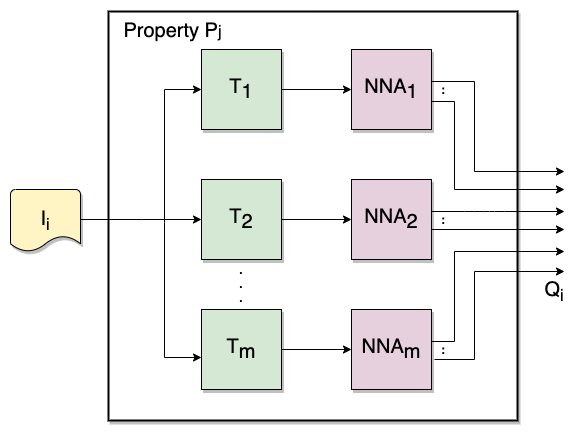
\includegraphics[width=90mm]{./images/property_transforms.png}}
\caption{Transformations of input based on properties}
\label{proptrans}
\end{figure}

This work explores multiple voting schemes\cite{blough}.  Some voting schemes involve probablistic algorithms such as likelihood weighting and maximum likelihood, while others involve ML algorithms.  Regardless of the voting algorithm, it was useful to construct and utilize a knowledgebase for storing detailed training and test results of the transformation NNs.  The knowledgebase was used in building or training voting algorithms. 
 
Applying our methodology for explainability involves the following steps:
\begin{itemize}
\item Explainable property discovery.
\item Define data transformations according to properties.
\item Transform training data.
\item Produce trained explainable property-specific NNs.
\item Build a Confidence Knowledgebase across the explainable properties.
\item Classification using the Confidence Knowledgebase.
\item Using a test dataset to provide feedback.
\end{itemize}

The steps in the methodology depicted in Fig.~\ref{xaimeth} and described further in this section.

\begin{figure}[htbp]
\centerline{\includegraphics[width=50mm]{xai-approach0.png}}
\caption{Steps in the XAI Methodology}
\label{xaimeth}
\end{figure}

The initial step is to discover explainable properties.  An explainable property is an attribute of a sample in the problem domain that may differentiate classes and provide a rationale for classification.  In the MNIST handwritten digit database, we pose explainable properties such as loops, lines, endpoints, and crossings.

Data transformation routines are next defined and implemented to represent a sample for classification according to the initial step's explainable properties.  A property may have one or more transforms.  Input to a transform is a sample to be classified, and the output of a transform routine will be the sample represented according to the property transform.  These transforms may be known algorithms of feature detection and extraction that may represent the properties or property characteristics.  In our example, we used digital image processing techniques related to the properties.  For example, a loop property may correspond to both closed or circular features. 

\begin{figure}[htbp]
\centerline{\includegraphics[width=100mm]{property-trans-training-set.png}}
\caption{Building Property Transform training sets}
\label{proptranstrain}
\end{figure}

We next generate a training dataset by submitting all elements from the original training set to the property transformations.  The output from each property transformation is stored separately for training each property transformation-specific NN.  The construction of the training sets for each property transformation for image $i$ is depicted in Fig. ~\ref{proptranstrain}, where the $i$th image is added to each collection of transformed training images.

The next step involves initializing unique NNs representing each property transformation and then using supervised ML techniques to train the NNs using only the output of that particular property transform and the original labels.  This results in a set of explainable property transforms and trained NNs that could be arranged in a pipeline as depicted in Fig.~\ref{widenn} that would allow an input image to be transformed and then classified according to each explainable property transform. 

\begin{figure}[htbp]
\centerline{\includegraphics[width=95mm]{property-nn.png}}
\caption{Property Transform trained NNs in a wide arrangement producing classification suggestions}
\label{widenn}
\end{figure}

After training, we utilize the pipeline depicted in Fig.~\ref{widenn} to process the training set and populate a confidence knowledgebase.  The knowledgebase stores the original training label, and each property transform classification from the property transform NNs.
We next devise a classification strategy using information from the knowledgebase.  We pose two in this work and suggest others for the future in TODO.
The first classification scheme is probabilistic.  In this scheme, we use the confidence knowledgebase to identify each NN's likelihood to classify the classes correctly.  Likelihoods are weighted and compared against the alternative classifications to provide confidence metrics for classifications.

After training, we utilize the pipeline depicted in Fig.~\ref{widenn} to process the training set and populate a confidence knowledgebase.  The knowledgebase stores the original training label, and each property transform classification from the property transform NNs.

\begin{figure}[htbp]
\centerline{\includegraphics[width=95mm]{property-nn-classification.png}}
\caption{The final classification pipeline with explainability}
\label{widennexp}
\end{figure}

We next devise a classification strategy using information from the knowledgebase.  The scheme will take as input the property transform classifications and output a final classification result as shown in Fig.~\ref{widennexp}.   The scheme must have the ability to tabulate votes from property transform NNs and intelligently select from potentially conflicting classifications.  We pose two schemes in this work and suggest others for the future in TODO.

The first classification scheme is probabilistic.  In this scheme, we use the confidence knowledgebase to identify each NN's likelihood of classifying the classes correctly.  Likelihoods are weighted, combined for like classifications, and then compared against the alternative classifications to provide confidence metrics for the potentially conflicting classifications.  This scheme may produce multiple classifications with confidence metrics if there is disagreement.

The second classification scheme utilizes the knowledgebase to train a NN to classify based on property transform results.  Using this scheme, we show very good results in our example.

Finally, when test data is presented to the pipeline, we evaluate the results and determine if more properties are needed.

Explanation for the final classification is provided in the property transform classification as depicted in Fig.~\ref{widennexp}.
 

\section{References}
\bibliographystyle{ieeetr}
\bibliography{references}

\vspace{12pt}


\end{document}
